%----------------------------------------------------------------------------------------
%	TESTING E PERFORMANCE
%----------------------------------------------------------------------------------------

\section{Testing e performance}
%intro + scalatest + server express w/postman

Il testing è un processo fondamentale nello sviluppo del software che mira a verificare se un'applicazione
funziona correttamente e soddisfa i requisiti specificati. Serve a individuare e correggere eventuali
errori o difetti nel codice, garantendo che il software sia affidabile, stabile e conforme alle aspettative degli utenti.

L'importanza di testing e performance engineering risiede nella garanzia della qualità del software.
Il testing assicura che il software sia privo di bug e funzioni correttamente, migliorando la fiducia
degli utenti e riducendo i costi legati a eventuali correzioni post-lancio. Le prestazioni,
d'altra parte, influenzano direttamente l'esperienza utente e la soddisfazione del cliente.
Un'applicazione lenta o instabile può respingere gli utenti.

\subsection{Scalatest}
ScalaTest è un framework di testing per il linguaggio di programmazione Scala.
È stato progettato per consentire una varietà di stili di testing, tra cui il testing unitario,
il testing di integrazione e il testing di accettazione.\\

All'interno del progetto, ScalaTest è stato utilizzato principalmente per il testing
unitario delle varie componenti del software lato Scala. Questo framework ha permesso agli
sviluppatori di scrivere test che verificano il comportamento delle singole unità di codice,
come classi e metodi, in isolamento. In questo modo, è stato possibile identificare e risolvere
eventuali bug o problemi nelle componenti del software in una fase precoce dello sviluppo.

\subsection{User App}
Testare un'applicazione web, specialmente con un framework come Svelte, può essere
impegnativo per diverse ragioni. Queste includono la complessità dei componenti,
l'uso di flussi di dati reattivi, la manipolazione del DOM, l'integrazione con servizi
esterni, la reattività dell'interfaccia utente su dispositivi diversi e il testing end-to-end.
Inoltre, gli aggiornamenti del framework richiedono test aggiuntivi per garantire la compatibilità.
In breve, il testing è cruciale per assicurare l'affidabilità di un'applicazione web, ma può essere
complesso a causa delle sfide uniche presentate dall'ambiente web e dall'architettura reattiva di Svelte.

\subsection{Postman}
Postman è stato utilizzato per effettuare vari test di integrazione, simulando le richieste
HTTP inviate dal client alle web API. Questo strumento ha permesso di verificare il corretto
funzionamento dei servizi REST e di identificare eventuali errori o problemi di comunicazione
tra il client e il server.\\

Sono state testate richieste sia nei confronti del server express che nei confronti del server
Akka HTTP. In particolare, sono state testate le richieste di login, di registrazione,
di visualizzazione delle colonnine e richieste di prenotazione o ricarica.\\

In seguito qualche esempio di richieste testate con Postman.

\begin{figure}[htbp]
    \centering
    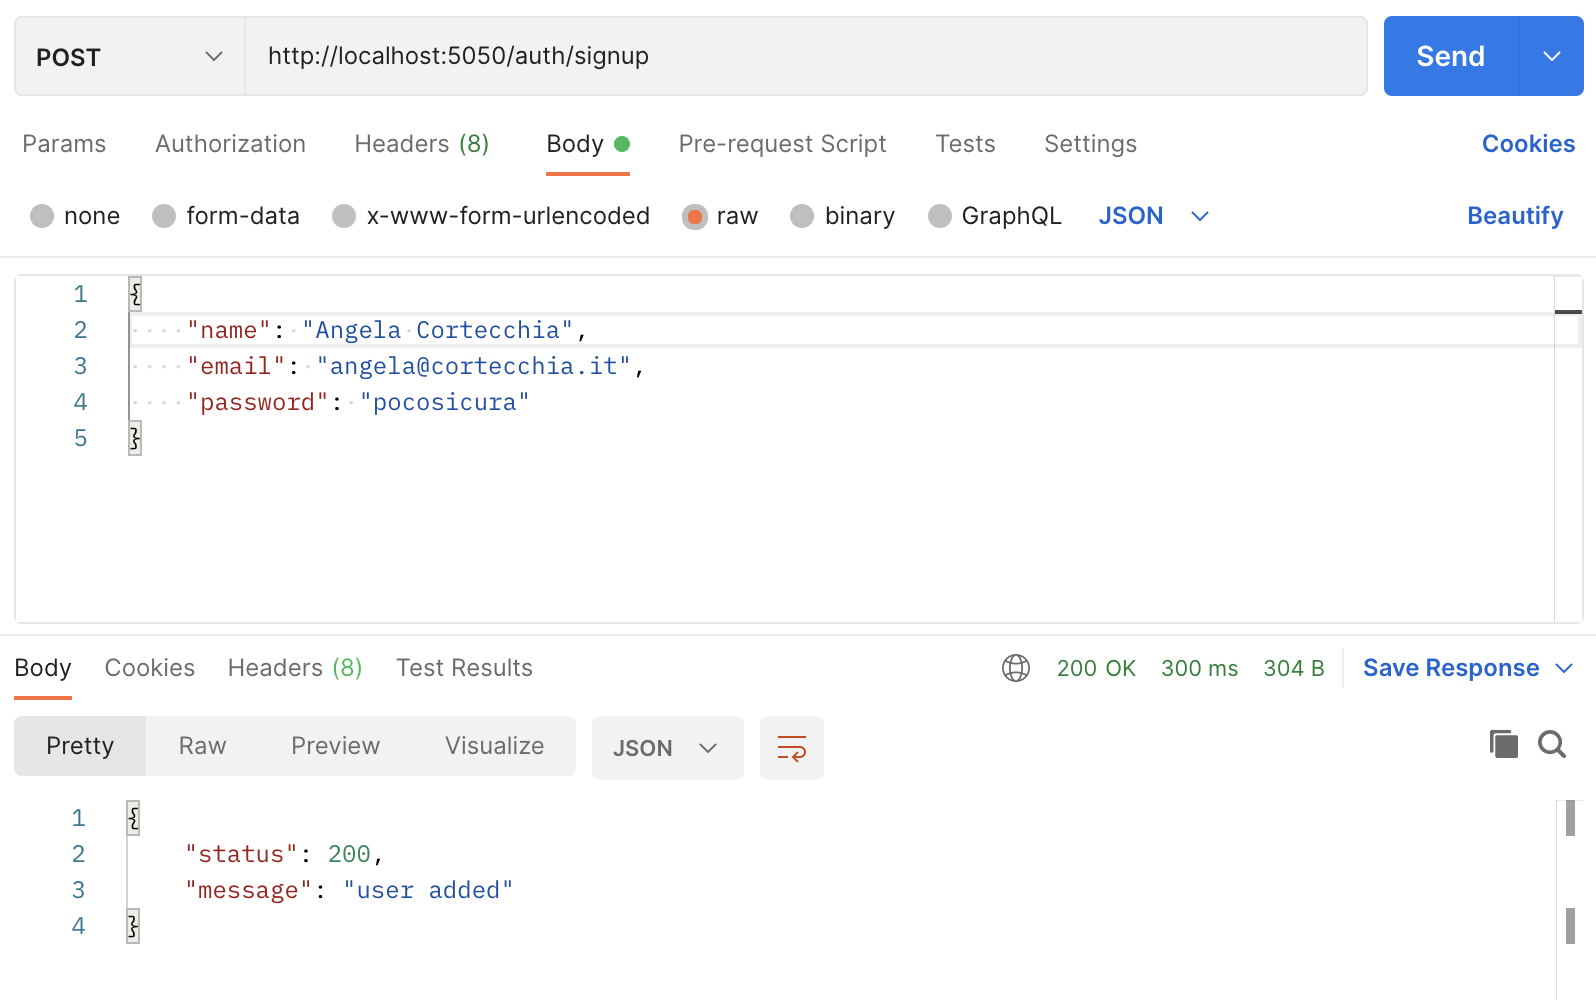
\includegraphics[width=\textwidth]{images/signupPostman.png}
    \caption{Richiesta di registrazione effettuata tramite Postman}
    \label{fig:signupPostman}
\end{figure}

\begin{figure}[htbp]
    \centering
    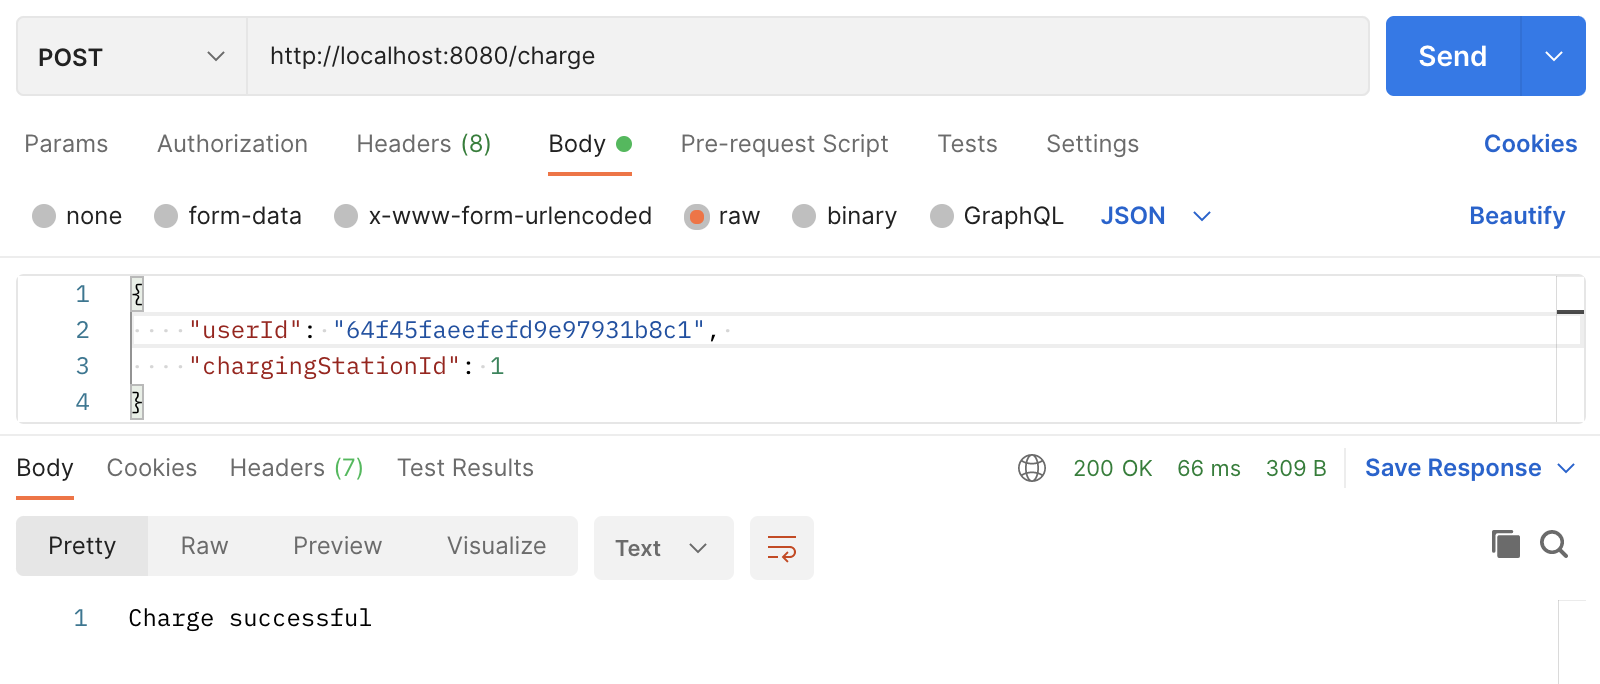
\includegraphics[width=\textwidth]{images/askCharge.png}
    \caption{Richiesta di ricarica presso una colonnina}
    \label{fig:askCharge}
\end{figure}

\begin{figure}[htbp]
    \centering
    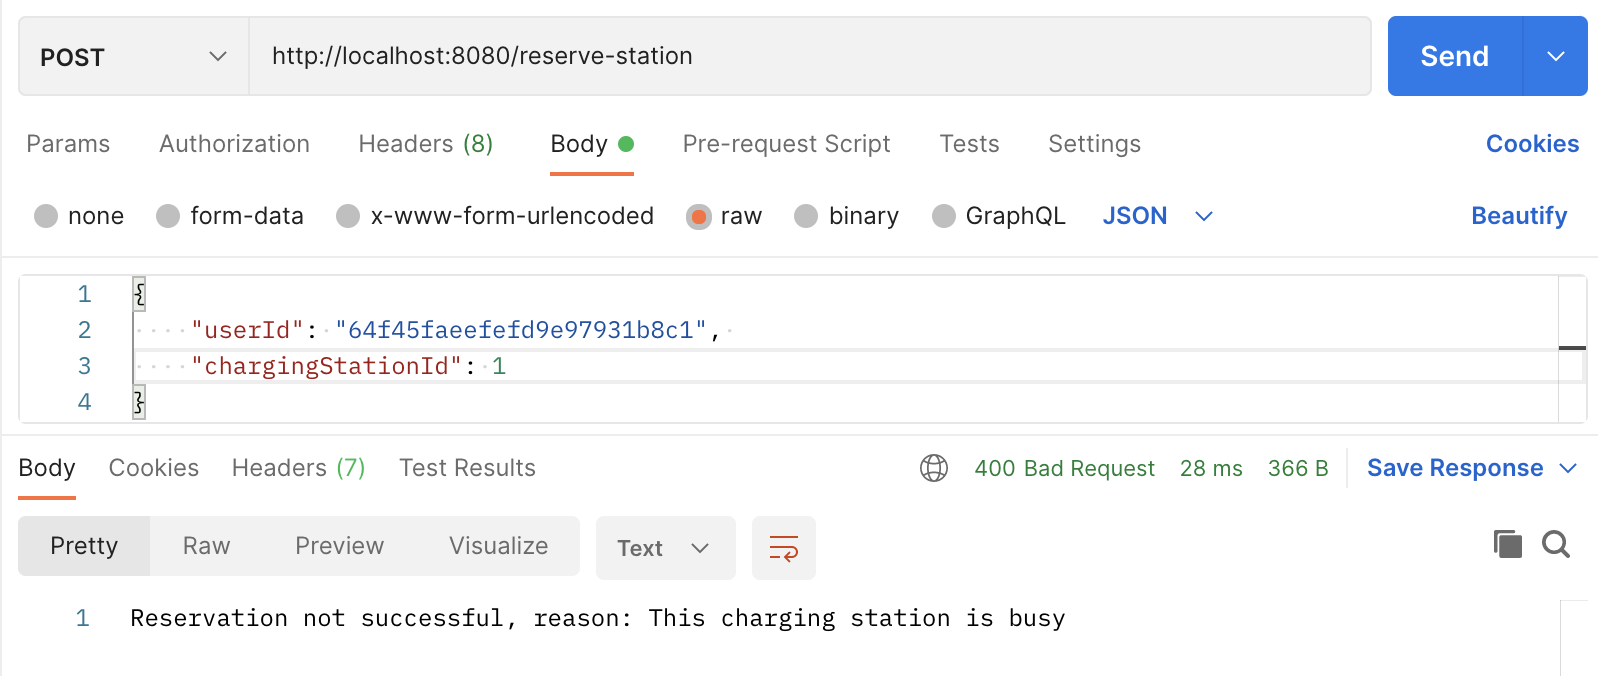
\includegraphics[width=\textwidth]{images/reserveNotOk.png}
    \caption{Richiesta di prenotazione di una colonnina non disponibile}
    \label{fig:reserveNotOk}
\end{figure}

\subsection{Charging Station Domain}
In seguito saranno discusse le modalità di testing delle componenti afferenti al Charging Station Domain.\\

\subsubsection{Unit Testing}
In ingegneria del software, per unit testing, test unitario[1] o collaudo unitario, si intende l'attività di collaudo di singole unità di un software. Per unità si intende normalmente il minimo componente di un programma dotato di funzionamento autonomo.\\
Nel caso di questo progetto, l'unità fondamentale da testare è la Charging Station, in quanto è l'unica che presenta un comportamento indipendente ed isolato dal resto delle componenti del sistema.\\
Per testare la Charging Station è stato utilizzato il framework ScalaTest, che permette di effettuare test di unità in modo semplice ed efficace, unito alle classi di test definite da Akka come \textbf{ActorTestKit}: esso fornisce
un actor system tipizzato che viene avviato al momento della creazione dei test e segue il ciclo di vita dell'intero test suite.\\

Abbiamo pertanto prima di tutto creato una classe di Test apposita per lo unit test dei componenti del nostro sistema:

\begin {lstlisting}[language=scala]
class TestService extends AnyWordSpec with BeforeAndAfterAll with Matchers:
  val testKit = ActorTestKit()
  given system: ActorSystem[Nothing] = testKit.system
  override def afterAll(): Unit = testKit.shutdownTestKit()
\end{lstlisting}

Questa classe può essere estesa da tutte le classi di test specifica che vogliamo creare.\\

L'actor test kit presente nella classe di test è stato utilizzato in due modi:

\begin{itemize}
    \item Per effettuare spawn degli attori da testare
    \item Per effettuare spawn di una \textbf{TestProbe}, ovvero un attore che permette di ricevere messaggi ed effettuare asserzioni su di essi
\end{itemize}

Segue, come esempio, un estratto del codice di test per il Charging Station Actor:

\begin {lstlisting}[language=scala]
class ChargingStationTest extends TestService:
  "A charging station" should {

    val chargingStation = ChargingStation(0, "Enel", "X Charging Station", 100, Position(44.17457186518429, 12.23658150624628))
    val chargeRequest = ChargeRequest("6d", 0)
    val reservation = Reservation("6d", 0)

    val sender = testKit.spawn(ChargingStationActor(chargingStation))

    "accept charging requests if free" in {
      val probe = testKit.createTestProbe[ChargeRequestResult]()
      sender ! ChargingStationEvents.Charge(chargeRequest, probe.ref)
      probe.expectMessage(ChargeRequestOk())
    }
  }

\end{lstlisting}


\subsubsection{Integration Testing}
Siccome gli altri componenti del Charging Station Domain sono strettamente accoppiati tra loro, il gruppo ha ritenuta più opportuna come metodologia di test per questi componenti l'integration testing.\\
Per realizzarlo è stata creata una main class che si occupa del setup e messa in funzione del cluster tramite file di configurazione. A questo punto, gli attori che compongono il cluster sono liberi di interagire e realizzare il comportamento da testare.\\
Per "scatenare" i comportamenti che si vogliono testare, è stato utilizzato il tool Postman, che permette di effettuare richieste HTTP verso i servizi REST esposti dal sistema.\\

%Esporre lo stato di funzionamento effettivo del sistema progettato ad elaborato concluso. Per ciascuna delle funzionalità salienti devono essere tabellate e discusse le performance riscontrate mediante opportuni test eseguiti in fase di validazione del progetto.\\

%I tempi di esecuzione/comunicazione devono essere accompagnati dalle caratteristiche dell'hardware sul quale è eseguito il software.\\


%Vincoli circa la lunghezza della sezione (escluse didascalie, tabelle, testo nelle immagini, schemi):

%\vspace{1cm}
%\begin{tabular}{l|rr}
%                    & Numero minimo di battute & Numero massimo di battute \\
%    \hline
%    1 componente & 2000                     & 3000                      \\
%    2 componenti & 2500                     & 4500                      \\
%    3 componenti & 3000                     & 6000                      \\
%    \hline
%\end{tabular}


\newpage